\section{Stacks and Heaps}
\label{sec:stacks_heaps}

\noindent
To further understand how our algorithms run, we must understand ligtly how memory is passed around in our programs.

\begin{Def}[Machine Code \& Compilation]

    Code is separated into two main areas of memory management, the program itself, and the data in transit during execution.
    The program itself is broken up such as follows:
    \begin{itemize}
        \item \textbf{Text Segment:} The part of the program which contains the executable code.
        \item \textbf{Data Segment:} The part of the program which contains global and static variables.
        \item \textbf{Machine Code:} The compiled code of the program, which is executed by the CPU.
    \end{itemize}

    \noindent
    Once the code compiles, we have two types of data to manage:
    \begin{itemize}
        \item \textbf{Initialized Data:} This is data that has been given a value before the program starts running, such as global variables.
        \item \textbf{Uninitialized Data:} This is data that has not been given a value before the program starts running, such as local variables.
    \end{itemize}
    \noindent
    Both types of data reside in memory at some address from which the CPU can access.
\end{Def}

\noindent
Let's talk about our first data structure, the stack:
\begin{Def}[Stack]

    A \textbf{stack data structure} is a collection of elements that follows a \textbf{Last In, First Out} (LIFO) principle. I.e., in a 
    stack of plates, the last added plate is the first one to be removed, not the middle or bottom/first plate.
    Each \textit{plate} in the stack is called a \textbf{stack frame}.
\end{Def}

\newpage

\noindent
This text does not concern assembly code or low-level programmming, so \underline{\textbf{do not}} get caught up on the specifics of this next example:
\begin{Example}[Assembly Code]
    Here is an assembly code example that demonstrates both initialized and uninitialized data. 
    Initialized data is placed in the `.data` section, while uninitialized data is placed in the `.bss` section:

    \begin{lstlisting}[language={[x86masm]Assembler}, numbers=none]
    section .data               ; Initialized data section
        num1    dd  7           ; num1 is initialized to 7
        num2    dd  3           ; num2 is initialized to 3

    section .bss                ; Uninitialized data section
        temp    resd 1          ; temp is reserved (uninitialized)
        result  resd 1          ; result is reserved (uninitialized)

    section .text               ; Code section
        global _start

    _start:
        mov eax, [num1]         ; Load num1 into eax
        mov [temp], eax         ; Store num1 in temp
        mov ebx, [num2]         ; Load num2 into ebx
        add eax, ebx            ; Add num2 to eax (eax = num1 + num2)
        mov [result], eax       ; Store the sum in result
    ; (Exit code omitted for brevity)
    \end{lstlisting}

    \noindent
    In this example, `num1` and `num2` are initialized before execution, while `temp` and `result` are uninitialized and only receive values during program execution.
\end{Example}

\noindent
Now let's look at how our programs utilize the stack:
\begin{Def}[Call Stack]

    A \textbf{call stack} is a stack which keeps track of function calls in a program as well as any local variables within such functions.
    
    \underline{This is why we say a variable is in \textbf{scope}}, as when a function is taken off the stack, or a new stack frame 
    is placed ontop, the variables in the previous or discarded stack frame are \textbf{no longer accessible}.
\end{Def}

\newpage 

\noindent
Let's illstrate this with the following diagram:

\begin{figure}[h]
    \centering
    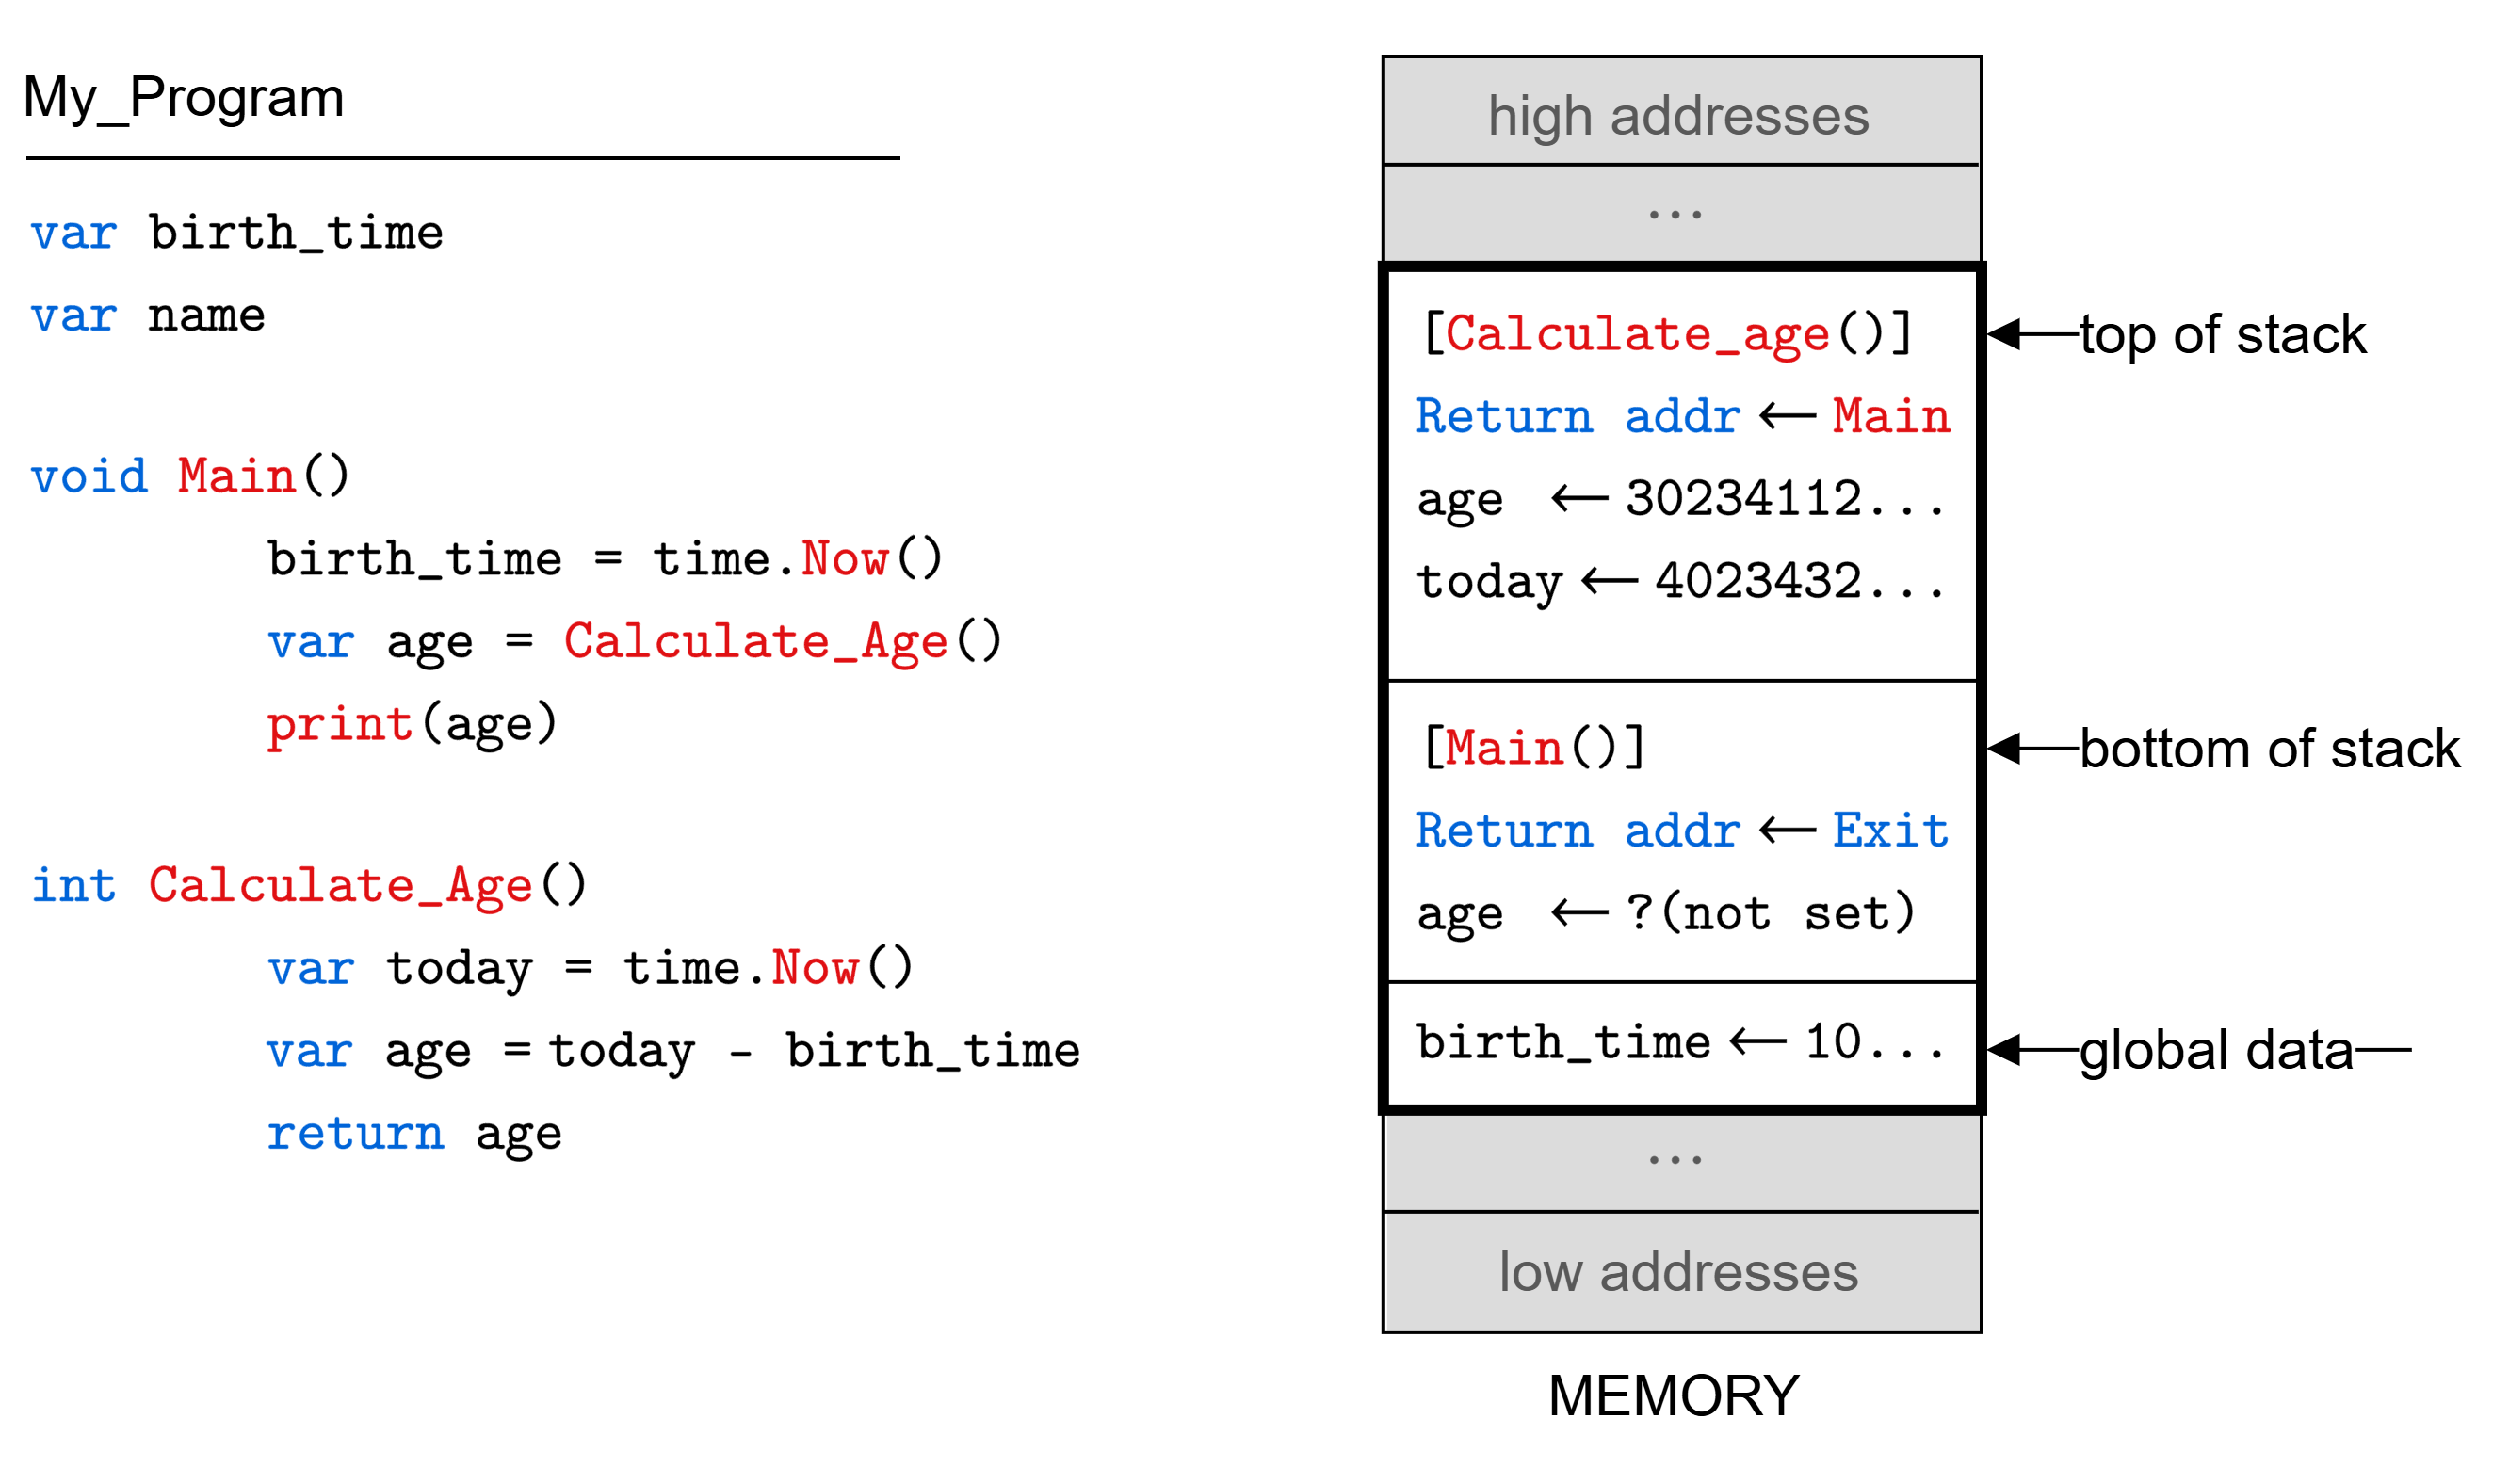
\includegraphics[width=0.8\textwidth]{./Sections/stacks_heaps/call_stack.png}
    \caption{Here is a simplified look at how memory manages the stack. On the left is our program written 
    in some abstract language, and on the right is the call stack in memory (simplified). 
    The program has a global `birth\_time' variable, which is intialized in the \texttt{Main} function. The \texttt{Main} function
    then calls the \texttt{Calculate\_Age} function which uses the `birth\_time' variable to calculate the `age' via the difference of 
    the current time and the `birth\_time.'
    Lookin at the memory, we see at the bottom of our memory contains global variables accessible to any frame. Next, is the bottom of the stack, containing a return address to exit 
    the program, while awaiting the result of the function call for `age'. The top of our stack contains another frame that we will return the value
    a new `age' (not the same as the one before) not accessible from the main function. This new frame also contains a new local variable `today.'
    Once this function returns, \texttt{Main} will have the result of its local variable `age.'. Concretely, the 
    `age' variable in both the \texttt{Main} and \texttt{Calculate\_Age} function are completely separate despite sharing the same \textit{name}.}
    \label{fig:call_stack}
\end{figure}

\newpage 
\noindent
To become more concrete each stack frame is actually broken up into multiple parts:
\begin{Def}[Stack Frame Anatomy]

Under the x86-32 calling convention, each function call creates a new \emph{stack frame} on the process's call stack. Two registers govern the layout of these frames:
\begin{itemize}
  \item \textbf{Base Pointer (BP/EBP):} Points to the base (i.e.\ ``bottom'') of the current function's stack frame.
  \item \textbf{Stack Pointer (SP/ESP):} Points to the ``top'' of the current function's stack frame, i.e., the next free byte where a push would land.
\end{itemize}

\noindent
When the program starts (or when a thread is created), the operating system \emph{reserves} a contiguous region of memory for the stack. By convention, the \emph{bottom} of that region lies at a higher address, 
and the stack ``grows downward'' toward lower addresses as data is pushed. If the stack pointer ever moves past the reserved limit---a \textbf{stack overflow} occurs.
\\

\noindent
A single \textbf{stack frame} itself is a contiguous block of memory in which the function stores:
\begin{itemize}
  \item \textbf{Parameters:} The arguments passed in by the caller (beyond what fits in registers, or always placed here by convention),  
  \item \textbf{Return Address:} The address to jump back to once this function returns,  
  \item \textbf{Old Base Pointer (Old EBP):} The caller's `EBP', saved so that on return we can restore the previous frame,  
  \item \textbf{Local Variables:} Space for any locals or temporaries that the function needs.  
\end{itemize}
Note that \emph{``New Base Pointer''} is simply the value of `ESP' after the old `EBP' has been pushed—this becomes the current `EBP' (i.e.\ the new base‐pointer register value), not a separate memory slot. Once a function returns, its entire frame is popped off the stack, so those local variables go ``out of scope'' and are no longer accessible.
\end{Def}

\noindent
On the next page we detail what exactly these offets are.

\newpage 

\noindent
Please observe the following table which illustrates the typical layout of a stack frame in x86-32 assembly language.
\begin{table}[h]
\centering
\resizebox{\textwidth}{!}{
\begin{tabular}{|c|c|l|}
\hline
\multicolumn{3}{|c|}{\textbf{High Addresses}} \\ \hline
\textbf{Contents}       & \textbf{Offset} & \textbf{Notes} \\
\hline
\emph{(Parameters 3, 4, \(\dots\))} & \(\mathit{EBP} + 16\), \(+20\), \(\dots\) & Third-and-onward arguments, if any. \\ 
Parameter 2            & \(\mathit{EBP} + 12\) & Second argument passed on stack. \\
Parameter 1            & \(\mathit{EBP} + 8\)  & First argument passed on stack. \\
Return Address         & \(\mathit{EBP} + 4\)  & Auto-pushed by the \texttt{call} instruction.\\
Old EBP (Saved BP)     & \(\mathit{EBP} + 0\)  & The caller's base pointer \\
\hline
\multicolumn{3}{|c|}{\textbf{Current Frame (locals/temporaries)}} \\ \hline
Local Variable 1        & \(\mathit{EBP} - 4\)  & First 4-byte local (or smallest slot). \\
Local Variable 2        & \(\mathit{EBP} - 8\)  & Next 4-byte local or part of a larger struct. \\
\(\dots\)                      & \( \vdots \)         &(additional locals at \(\mathit{EBP} - 12,\ -16,\ \dots\)) \\
\hline
\multicolumn{3}{|c|}{\textbf{Low Addresses}} \\ \hline
\end{tabular}
}
\caption{Typical x86-32 Stack-Frame Layout, where offsets are typically a multiple of 4 bytes. The \textit{EBP} register points to the base of the current stack frame, and offsets are calculated relative to it. The stack grows downwards, so higher offsets correspond to lower memory addresses.}
\end{table}

